\documentclass[12pt]{article}

	\usepackage[utf8]{inputenc}
	\usepackage[brazilian]{babel}
	\usepackage{hyperref}
	\usepackage{lipsum}
	\usepackage{geometry}
	\usepackage[skip=5pt plus1pt, indent=20pt]{parskip}
	\usepackage{indentfirst}
	\usepackage{amsthm,amssymb,amsmath}
	\usepackage{minted}
	\usepackage{graphicx}
	
	\geometry{left=3cm, top=3cm, right=2cm, bottom=2cm}
	
	\title{\textbf{Sistemas Operacionais - TP1\\
	\large getcnt syscall on xv6}}
	\author{\textbf{Matheus Flávio Gonçalves Silva - 2020006850}}
	\date{\parbox{\linewidth}{\centering%
    Universidade Federal de Minas Gerais (UFMG)\endgraf
    Belo Horizonte - MG - Brasil\endgraf\bigskip
    \href{mailto:matheusfgs@ufmg.br}{matheusfgs@ufmg.br}}}
	
	\begin{document}

\maketitle

%%%%%%%%%%%%%%%%%%%%%%%%%%%%%%%%%%%%%%%%%%%%%%%%%%%%%%%%%%%%%%%%%%%%%%%%%%%%%%

\section{Introdução}
\par Neste trabalho é utilizado sistema operacional de aprendizado \textbf{XV6}. O sistema em questão é feito de modo a abranger diversos conceitos chaves \textbf{UNIX}, e, para utilizá-lo, é necessário compilar os arquivos fontes com a utilização do processador emulado \textbf{QEMU}
%%%%%%%%%%%%%%%%%%%%%%%%%%%%%%%%%%%%%%%%%%%%%%%%%%%%%%%%%%%%%%%%%%%%%%%%%%%%%%
\section{Preparação}

\par Para executar o sistema e realizar o trabalho, é necessário seguir o seguinte passo-a-passo:

\subsection{Instalação de dependências}
\par A instalação das dependências necessária é feita em ambiente Linux de base Ubuntu (Linux Mint) com a execução do seguinte comando no terminal:

\begin{minted} [
	frame=lines,
	framesep=2mm,
	baselinestretch=1.2,
	fontsize=\footnotesize,
	linenos,
	breaklines
	]{bash}
sudo apt-get install git build-essential gdb-multiarch qemu-system-misc gcc-riscv64-linux-gnu binutils-riscv64-linux-gnu
\end{minted}

\subsection{Download do XV6}
\par O Download dos arquivos do XV6 é simplesmente feito por meio da cópia ou fork do repositório do projeto original do MIT. Para isso, basta simplesmente executar o comando a seguir caso prefira clonar o repositório
\begin{minted} [
	frame=lines,
	framesep=2mm,
	baselinestretch=1.2,
	fontsize=\footnotesize,
	linenos,
	breaklines
	]{bash}
# Clone
git clone https://github.com/mit-pdos/xv6-riscv.git
\end{minted}

\par Caso prefira fazer um fork, basta selecionar a opção na página do Github.

\subsection{Execução}
\par A execução do sistema, que é feita de foram similar à execução de um terminal padrão do linux, é feita por meio do comando:
\begin{minted} [
	frame=lines,
	framesep=2mm,
	baselinestretch=1.2,
	fontsize=\footnotesize,
	linenos,
	breaklines
	]{bash}
make qemu
\end{minted}

Ao executar o comando acima, é aberto um emulador de terminal que aceita os comandos definidos no sistema.
%%%%%%%%%%%%%%%%%%%%%%%%%%%%%%%%%%%%%%%%%%%%%%%%%%%%%%%%%%%%%%%%%%%%%%%%%%%%%%

\section{Implementação}

\subsection{Estrutura de Dados}
\par A Estrutura da Dados para manter a quantidade de chamadas de cada função é simplesmente um vetor de 22 posições inicializado com 0 em cada posição, cada índice armazenando a quantidade de execuções do comando com o pid correspondente ao índice + 1.

\begin{minted} [
	frame=lines,
	framesep=2mm,
	baselinestretch=1.2,
	fontsize=\footnotesize,
	linenos,
	breaklines
	]{C}
//proc.c
int sys_cnt[22] = {0};
\end{minted}

\subsection{Atualização da Estrutura de Dados}
\par Tendo em mente a Estrutura de Dados, essa variável é simplesmente utilizada como sendo uma variável global que pode ser acessada por todo código que importe "proc.h":

\begin{minted} [
	frame=lines,
	framesep=2mm,
	baselinestretch=1.2,
	fontsize=\footnotesize,
	linenos,
	breaklines
	]{C}
//Exemplo do sysfile.c atualizando as chamadas do comando "dup"
extern int sys_cnt[22];
	
// Fetch the nth word-sized system call argument as a file descriptor
// and return both the descriptor and the corresponding struct file.
static int
@@ -57,6 +59,8 @@ sys_dup(void)
struct file *f;
int fd;
	
sys_cnt[SYS_dup - 1]++; //Atualização da quantidade de chamas do processo de pid referente ao dup
\end{minted}

\par Todos os processos são atualizados da mesma forma, apenas alterando o valor atribuído à posição do vetor que é manipulada.

\par Foi feito também o include da lib syscall.h para utilizar os defines lá declarados tornando mais fácil entender os pids ao não utilizar os pids numéricos diretamente.

\subsection{Implementação da função}
\par A implementação da função em si segue os padrões definidos anteriormente no projeto, levando como base, por exemplo, a chamada "argint" para pegar o pid passado como parâmetro e utilizando manipulações simples de inteiros com o retorno da posição do vetor referente à quantidade de chamadas do processo passado como parâmetro.

\par Essa implementação é feita como segue em \textbf{sysfile.c}:
\begin{minted} [
	frame=lines,
	framesep=2mm,
	baselinestretch=1.2,
	fontsize=\footnotesize,
	linenos,
	breaklines
	]{C}
uint64
sys_getcnt(void)
{
	sys_cnt[SYS_getcnt - 1]++;

	int sys_ID;
	argint(0, &sys_ID); //argfd mostra como pegar um argumento int
	sys_ID--;
	return sys_cnt[sys_ID];
}\end{minted}

\subsection{Impressão do comando}
\par Por fim, deve-se tratar da impressão do comando feita de acordo com o passado na especificação do TP. Isso é feito um arquivo criado à parte \textbf{getcnt.c}:

\begin{minted}[
    frame=lines,
    framesep=2mm,
    baselinestretch=1.2,
    fontsize=\footnotesize,
    linenos,
    breaklines
    ]{C}
#include "kernel/types.h"
#include "kernel/stat.h"
#include "user/user.h"

extern int sys_cnt[22];

int
main(int argc, char *argv[])
{
	if(argc < 2){
		fprintf(2, "usage: getcnt pid...\n");
	    exit(1);
	}

  	int sys_ID = atoi(argv[1]);
  	int id_cnt = getcnt(sys_ID);

  	fprintf(2, "syscall %s has been called %d times\n", argv[1], id_cnt);

  	exit(0);
}
\end{minted}
%%%%%%%%%%%%%%%%%%%%%%%%%%%%%%%%%%%%%%%%%%%%%%%%%%%%%%%%%%%%%%%%%%%%%%%%%%%%%%
\section{Teste}
\par O teste da implementação foi feito seguindo uma rotina simulando a utilização simples de um usuário interagindo com o terminal, sendo realizados uma verificação de contagem, a criação de 4 pastas, a contagem do comando mkdir, a contagem do comando read, e a contagem do getcnt finalizando a rotina de testes.
\begin{figure}[hb]
	\centering
	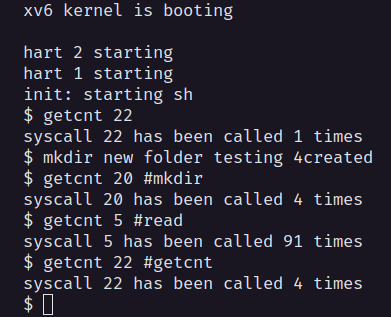
\includegraphics[scale=0.8]{./teste.png}
	\caption{Rotina de testes simulando usuário}
\end{figure}
\end{document}
